% cd /storage/emulated/0/Documents/documents/latex/1920/Grade-8/3rd/triangle-congruence && pdflatex act-triangle-congruence.tex && termux-open act-triangle-congruence.pdf  


\documentclass[10pt]{article}
\usepackage[legalpaper, right=1mm, left=1mm, top=1mm, bottom=1mm]{geometry}
\usepackage{tikz} 

\begin{document} 
\centering
\begin{tikzpicture} 
%1
\node[inner sep=0] at (-9, 8) {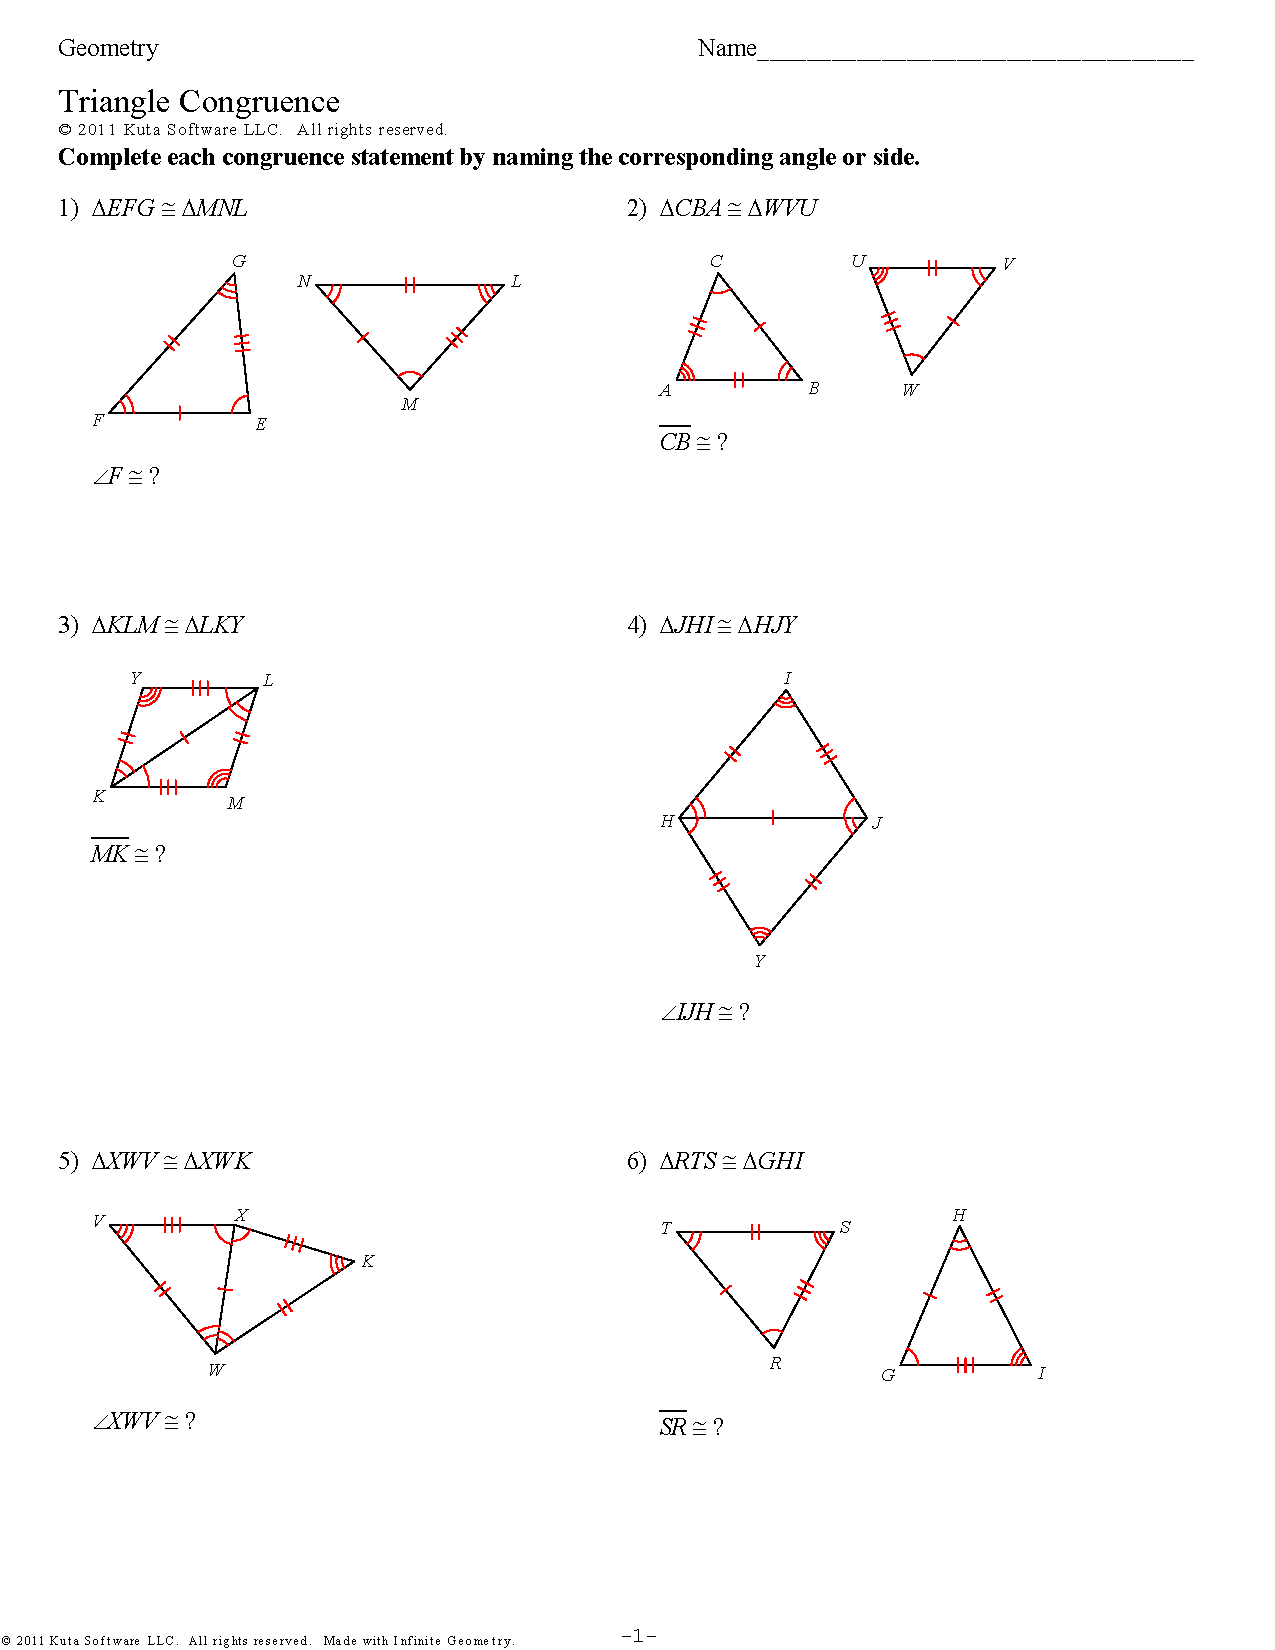
\includegraphics[page=1, width=0.5\textwidth, height = 0.48\textheight]{kuta-triangle-congruence.pdf}}; 

%2
\node[inner sep=0] at (3, 8) {\includegraphics[page=2, width=0.5\textwidth, height = 0.48\textheight]{kuta-triangle-congruence.pdf}}; 

%3
\node[inner sep=0] at (-9, -10) {\includegraphics[page=3, width=0.5\textwidth, height = 0.48\textheight]{kuta-triangle-congruence.pdf}}; 

%4
\node[inner sep=0] at (3, -10) {\includegraphics[page=4, width=0.5\textwidth, height = 0.48\textheight]{kuta-triangle-congruence.pdf}}; 

\end{tikzpicture} 
\end{document}




